% !TeX program = xelatex
\documentclass[a4paper,10pt]{article}

% ============================================================================
% កញ្ចប់បណ្ណាល័យ (Packages) – តាមលំនាំ NGS Preah Krasang Scenario
% ============================================================================
\usepackage[a4paper, left=0.95cm, right=0.95cm, top=0.80cm, bottom=0.90cm, footskip=0.45cm]{geometry}
\usepackage{amsmath, amssymb}
\usepackage{unicode-math}
\usepackage{fontspec}
\usepackage{array, longtable, multirow, colortbl}
\usepackage[table]{xcolor}
\usepackage{enumitem}
\usepackage{pifont}
\usepackage{fancyhdr}
\usepackage{tikz}
\usetikzlibrary{calc, arrows.meta, decorations.markings, decorations.pathreplacing, patterns, babel}

% LaTeX 2025 + longtable v4.24 compatibility guard
\makeatletter
\let\@expl@@@mark@update@singlecol@structures@@\relax
\makeatother

% ============================================================================
% ការកំណត់ពុម្ពអក្សរ (Cross-Platform Fonts Configuration)
% ============================================================================
\providecommand{\NGSFindFonts}{%
  \IfFileExists{C:/Windows/Fonts/cambria.ttc}{%
    \def\NGSSysPath{C:/Windows/Fonts/}%
    \def\NGSUserPath{C:/Users/KIT/AppData/Local/Microsoft/Windows/Fonts/}%
  }{%
    \IfFileExists{./fonts/KhmerOSsiemreap.ttf}{\def\NGSSysPath{./fonts/}\def\NGSUserPath{./fonts/}}{%
    \IfFileExists{../fonts/KhmerOSsiemreap.ttf}{\def\NGSSysPath{../fonts/}\def\NGSUserPath{../fonts/}}{%
    \IfFileExists{../../fonts/KhmerOSsiemreap.ttf}{\def\NGSSysPath{../../fonts/}\def\NGSUserPath{../../fonts/}}{%
    \IfFileExists{../../../fonts/KhmerOSsiemreap.ttf}{\def\NGSSysPath{../../../fonts/}\def\NGSUserPath{../../../fonts/}}{%
    \IfFileExists{../../../../fonts/KhmerOSsiemreap.ttf}{\def\NGSSysPath{../../../../fonts/}\def\NGSUserPath{../../../../fonts/}}{%
    \IfFileExists{../../../../../fonts/KhmerOSsiemreap.ttf}{\def\NGSSysPath{../../../../../fonts/}\def\NGSUserPath{../../../../../fonts/}}{%
    \IfFileExists{../../../../../../fonts/KhmerOSsiemreap.ttf}{\def\NGSSysPath{../../../../../../fonts/}\def\NGSUserPath{../../../../../../fonts/}}{%
      \def\NGSSysPath{../../../../../../../fonts/}\def\NGSUserPath{../../../../../../../fonts/}%
    }}}}}}}%
  }%
}
\NGSFindFonts

\setmathfont[
  Path={\NGSSysPath},
  FontIndex=1,
  Scale=1.02
]{cambria.ttc}

\defaultfontfeatures{Ligatures=TeX}

\setmainfont[
  Path={\NGSUserPath},
  Extension=.ttf,
  Script=Khmer,
  BoldFont={KhmerOSsiemreap},
  BoldFeatures={FakeBold=1.8},
  ItalicFont={KhmerOSsiemreap},
  ItalicFeatures={FakeSlant=0.25},
  BoldItalicFont={KhmerOSsiemreap},
  BoldItalicFeatures={FakeBold=1.8, FakeSlant=0.25}
]{KhmerOSsiemreap}

\newfontfamily\muol[
  Path={\NGSUserPath},
  Extension=.ttf,
  Script=Khmer
]{KhmerOSmuollight}

\newfontfamily\TimesEn[
  Path={\NGSSysPath},
  Extension=.ttf,
  Scale=1.00,
  BoldFont={timesbd},
  ItalicFont={timesi},
  BoldItalicFont={timesbi}
]{times}

\newfontfamily\NagaBold[
  Path={\NGSUserPath},
  Extension=.ttf
]{AKbalthom Naga Bold}

\newfontfamily\CalibriFont[
  Path={\NGSSysPath},
  Extension=.ttf
]{calibri}

\newfontfamily\CourierBullet[
  Path={\NGSSysPath},
  Extension=.ttf
]{cour}
\newcommand{\wcirc}{{\CourierBullet\fontsize{9.5pt}{11pt}\selectfont o}}

\XeTeXlinebreaklocale "km"
\XeTeXlinebreakskip = 0pt plus 1pt minus 0.1pt

% ============================================================================
% ការកំណត់ពណ៌ និងទម្រង់ទំព័រ (Colors & Page Style)
% ============================================================================
\definecolor{stepgray}{HTML}{D9D9D9}
\definecolor{headgray}{HTML}{F2F2F2}
\definecolor{boxgray}{HTML}{D9D9D9}
\definecolor{darkred}{HTML}{C00000}
\definecolor{red5e}{HTML}{FF0000}

\pagestyle{fancy}
\fancyhf{}
\renewcommand{\headrulewidth}{0pt}
\fancyfoot[L]{\fontsize{8.0pt}{10pt}\selectfont អនុវិទ្យាល័យព្រះក្រសាំង \en{|} សេណារីយ៉ូ ៥០ នាទី៖ ២.៣ វិធីចែកស្វ័យគុណមាននិទស្សន្តរ៉ឺឡាទីប \en{|} ១៦ វិច្ឆិកា ២០២៦}
\fancyfoot[R]{\CalibriFont\fontsize{10.5pt}{12pt}\selectfont\thepage}

\setlength{\parindent}{0pt}
\setlength{\parskip}{0pt}
\setlength{\tabcolsep}{3.5pt}
\renewcommand{\arraystretch}{1.08}

\newcolumntype{L}[1]{>{\raggedright\arraybackslash}p{#1}}

% ============================================================================
% ម៉ាក្រូជំនួយ (Helper Macros)
% ============================================================================
\newcommand{\en}[1]{{\TimesEn #1}}
\newcommand{\enbf}[1]{{\TimesEn\textbf{#1}}}
\newcommand{\unit}[1]{\,\text{\en{#1}}}
\newcommand{\fiveE}[1]{{\NagaBold\fontsize{9.5pt}{13pt}\selectfont\textcolor{red5e}{#1}}}
\newcommand{\timenote}[1]{\textcolor{darkred}{\textit{#1}}}
\newcommand{\cnum}[1]{{\fontsize{10pt}{11.5pt}\selectfont\ding{\numexpr181+#1\relax}}}
\newcommand{\ditem}{\tikz[baseline=-0.5ex]\fill (0,0.38ex) -- (0.38ex,0) -- (0,-0.38ex) -- (-0.38ex,0) -- cycle;\hspace{0.25em}}

% ============================================================================
% រូបផ្ទៀងផ្ទាត់រហ័ស & ប្លង់ក្ដារខៀន (B&W TikZ Diagrams)
% ============================================================================
\newcommand{\figBoardLayoutPOW}{%
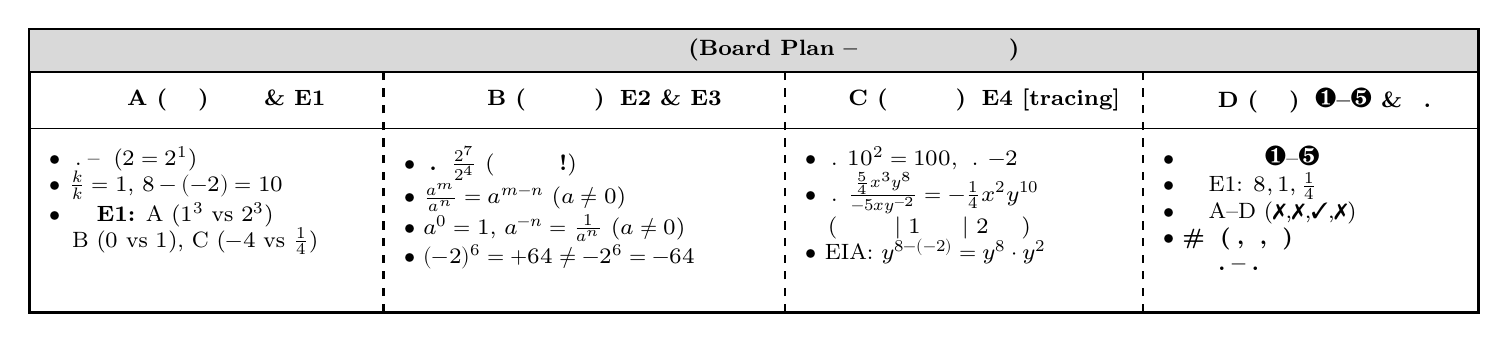
\begin{tikzpicture}[scale=1.0, every node/.style={font=\footnotesize, text=black}]
  \draw[black, line width=1.1pt, fill=white] (0,0) rectangle (18.4, 3.60);
  \draw[black, line width=0.8pt, fill=stepgray] (0, 3.06) rectangle (18.4, 3.60);
  \node at (9.20, 3.33) {\textbf{ប្លង់គ្រប់គ្រងក្ដារខៀន ៤ តំបន់ (\en{Board Plan} -- រក្សាទុកពីដើមដល់ចប់ម៉ោង)}};
  \draw[black, line width=0.75pt, dashed] (4.50, 0) -- (4.50, 3.06);
  \draw[black, line width=0.75pt, dashed] (9.60, 0) -- (9.60, 3.06);
  \draw[black, line width=0.75pt, dashed] (14.15, 0) -- (14.15, 3.06);
  \draw[black, line width=0.6pt] (0, 2.34) -- (18.4, 2.34);
  % តំបន់ A
  \node[align=center] at (2.25, 2.70) {\textbf{តំបន់ \en{A} (ឆ្វេង)៖ រំលឹក \& \en{E1}}};
  \node[anchor=north west, align=left] at (0.14, 2.24) {$\bullet$ ៦.ក--គ ($2=2^1$)\\ $\bullet$ $\frac{k}{k}=1$, $8-(-2)=10$\\ $\bullet$ \textbf{ទាយ \en{E1}:} \en{A} ($1^3$ vs $2^3$)\\ \quad \en{B} ($0$ vs $1$), \en{C} ($-4$ vs $\frac{1}{4}$)};
  % តំបន់ B
  \node[align=center] at (7.05, 2.70) {\textbf{តំបន់ \en{B} (កណ្ដាលឆ្វេង)៖ \en{E2} \& \en{E3}}};
  \node[anchor=north west, align=left] at (4.64, 2.24) {$\bullet$ \textbf{២.៣} $\frac{2^7}{2^4}$ (\textbf{៧ កត្តាពេញ!})\\ $\bullet$ $\frac{a^m}{a^n}=a^{m-n}$ ($a\neq 0$)\\ $\bullet$ $a^0=1$, $a^{-n}=\frac{1}{a^n}$ ($a\neq 0$)\\ $\bullet$ $(-2)^6=+64 \neq -2^6=-64$};
  % តំបន់ C
  \node[align=center] at (11.875, 2.70) {\textbf{តំបន់ \en{C} (កណ្ដាលស្ដាំ)៖ \en{E4 [tracing]}}};
  \node[anchor=north west, align=left] at (9.74, 2.24) {$\bullet$ ក. $10^2=100$, ខ. $-2$\\ $\bullet$ គ. $\frac{\frac{5}{4}x^3y^8}{-5xy^{-2}} = -\frac{1}{4}x^2y^{10}$\\ \quad (ស៊ុមទ្វេ \textbar{} $1$ ជាន់ \textbar{} $2$ ជាន់)\\ $\bullet$ \en{EIA}: $y^{8-(-2)}=y^8\cdot y^2$};
  % តំបន់ D
  \node[align=center] at (16.275, 2.70) {\textbf{តំបន់ \en{D} (ស្ដាំ)៖ \cnum{1}--\cnum{5} \& ទំ.២៥}};
  \node[anchor=north west, align=left] at (14.28, 2.24) {$\bullet$ ផ្ទាំងធនាគារ \cnum{1}--\cnum{5}\\ $\bullet$ បិទ \en{E1}: $8, 1, \frac{1}{4}$\\ $\bullet$ កាត \en{A--D} (\ding{55},\ding{55},\ding{51},\ding{55})\\ $\bullet$ \textbf{\#៧ (គ, ឃ, ច)}\\ \quad អាន \textbf{៤.១--៤.២}};
\end{tikzpicture}}

\newcommand{\figScenarioRefPOW}{%
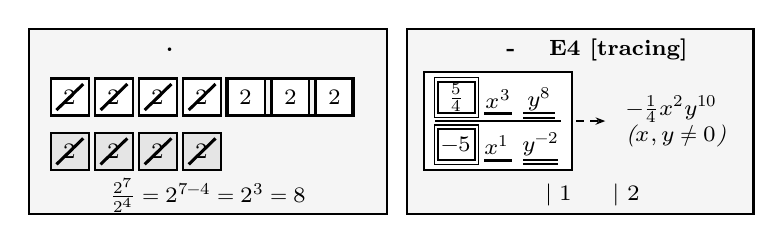
\begin{tikzpicture}[scale=1.0, every node/.style={font=\footnotesize, text=black}]
  % ឆ្វេង៖ គំរូបន្ទះ 1:1 ៧ កត្តាពេញ (2^7 / 2^4)
  \begin{scope}[shift={(0,0)}]
    \draw[black, line width=0.9pt, fill=gray!8] (0,0) rectangle (4.55, 2.35);
    \node at (2.275, 2.08) {\textbf{កែទំ.១៦៖ ពេញ ៧ កត្តា}};
    \foreach \i in {0,...,6}{
      \draw[black, line width=0.8pt, fill=white] (0.28+\i*0.56, 1.25) rectangle (0.76+\i*0.56, 1.72);
      \node at (0.52+\i*0.56, 1.485) {$2$};
    }
    \foreach \i in {0,...,3}{
      \draw[black, line width=0.8pt, fill=gray!20] (0.28+\i*0.56, 0.56) rectangle (0.76+\i*0.56, 1.03);
      \node at (0.52+\i*0.56, 0.795) {$2$};
      \draw[black, line width=1.1pt] (0.35+\i*0.56, 1.32) -- (0.69+\i*0.56, 1.65);
      \draw[black, line width=1.1pt] (0.35+\i*0.56, 0.63) -- (0.69+\i*0.56, 0.96);
    }
    \draw[black, line width=1.35pt] (2.52, 1.25) rectangle (4.12, 1.72);
    \node at (2.275, 0.24) {$\frac{2^7}{2^4} = 2^{7-4} = 2^3 = 8$};
  \end{scope}
  % ស្ដាំ៖ គំរូកាត E4 [tracing] ស-ខ្មៅ
  \begin{scope}[shift={(4.80,0)}]
    \draw[black, line width=0.9pt, fill=gray!8] (0,0) rectangle (4.40, 2.35);
    \node at (2.20, 2.08) {\textbf{កូដ ស-ខ្មៅ \en{E4 [tracing]}}};
    \draw[black, line width=0.85pt, fill=white] (0.22, 0.56) rectangle (2.10, 1.80);
    \draw[black, line width=0.85pt] (0.36, 1.18) -- (1.96, 1.18);
    \draw[black, line width=0.7pt] (0.40, 1.28) rectangle (0.86, 1.68);
    \draw[black, line width=0.4pt] (0.35, 1.23) rectangle (0.91, 1.73);
    \node at (0.63, 1.48) {$\frac{5}{4}$};
    \node at (1.16, 1.46) {$x^3$};
    \draw[black, line width=1.1pt] (0.98, 1.27) -- (1.34, 1.27);
    \node at (1.68, 1.46) {$y^8$};
    \draw[black, line width=0.75pt] (1.48, 1.28) -- (1.88, 1.28) (1.48, 1.22) -- (1.88, 1.22);
    \draw[black, line width=0.7pt] (0.40, 0.68) rectangle (0.86, 1.08);
    \draw[black, line width=0.4pt] (0.35, 0.63) rectangle (0.91, 1.13);
    \node at (0.63, 0.88) {$-5$};
    \node at (1.14, 0.88) {$x^1$};
    \draw[black, line width=1.1pt] (0.98, 0.68) -- (1.34, 0.68);
    \node at (1.70, 0.88) {$y^{-2}$};
    \draw[black, line width=0.75pt] (1.48, 0.69) -- (1.92, 0.69) (1.48, 0.63) -- (1.92, 0.63);
    \draw[black, line width=0.9pt, densely dashed, -{Stealth[length=3.5pt]}] (2.15, 1.18) -- (2.52, 1.18);
    \node[align=left] at (3.42, 1.18) {$-\frac{1}{4} x^2 y^{10}$\\ \textit{($x,y\neq 0$)}};
    \node at (2.20, 0.24) {ស៊ុមទ្វេ \textbar{} $1$ ជាន់ \textbar{} $2$ ជាន់};
  \end{scope}
\end{tikzpicture}}

\begin{document}
\fontsize{9.4pt}{13.6pt}\selectfont

% ============================================================================
% ក្បាលទំព័រ (Header & Metadata)
% ============================================================================
\begin{center}
{\muol\fontsize{10.6pt}{14pt}\selectfont សេណារីយ៉ូនៃការបង្រៀន \enbf{(Teaching Scenario -- 50 min)}}
\end{center}
\vspace{2pt}

\noindent{\setlength{\tabcolsep}{4pt}%
\begin{tabular}{|L{1.75cm}|L{6.65cm}|L{1.85cm}|L{7.55cm}|}
\hline
\rowcolor{headgray}
\textbf{សាលារៀន៖} & អនុវិទ្យាល័យព្រះក្រសាំង (កំពង់ស្វាយ--កំពង់ធំ) & \textbf{មុខវិជ្ជា៖} & គណិតវិទ្យា ថ្នាក់ទី៨ (ពីជគណិត — មេរៀនទី២ ស្វ័យគុណ) \\
\hline
\textbf{មេរៀន៖} & \textbf{២.៣. វិធីចែកស្វ័យគុណមាននិទស្សន្តរ៉ឺឡាទីប} & \textbf{រយៈពេល៖} & \textcolor{darkred}{\textbf{១ ម៉ោងសិក្សា (៥០ នាទី)}} \textbullet\ ទំ.១៦--១៨, ២៥ \\
\hline
\textbf{គ្រូបង្រៀន៖} & ហុក ប៊ុនថែន & \textbf{កាលបរិច្ឆេទ៖} & ចន្ទ ៧កើត កត្តិក ២៥៧០ (១៦ វិច្ឆិកា ២០២៦) \\
\hline
\end{tabular}}

\vspace{4pt}
{\muol ផ្នែកទី ១៖ លំដាប់ឈុតឆាកបង្រៀន ៥០ នាទី \enbf{(}៨ ឈុតលម្អិត\enbf{)}}
\vspace{2pt}

% ============================================================================
% ផ្នែកទី ១៖ តារាងឈុតឆាក (8 Chronological Scenes = 50 min, Granular Sub-Rows)
% ============================================================================
\begin{longtable}{|c|L{2.75cm}|c|L{7.65cm}|L{4.45cm}|}
\hline
\rowcolor{stepgray}
\textbf{ម៉ោង} & \textbf{ឈុត / ជំហាន \enbf{5E}} & \textbf{នាទី} & \textbf{សកម្មភាពបង្រៀន និងសំណួរ--ចម្លើយគំរូ (គ្រូ--សិស្ស)} & \textbf{សម្ភារៈ និងកំណត់ចំណាំ / \enbf{Warrant}} \\
\hline
\endfirsthead
\hline
\rowcolor{stepgray}
\textbf{ម៉ោង} & \textbf{ឈុត / ជំហាន \enbf{5E}} & \textbf{នាទី} & \textbf{សកម្មភាពបង្រៀន និងសំណួរ--ចម្លើយគំរូ (គ្រូ--សិស្ស)} & \textbf{សម្ភារៈ និងកំណត់ចំណាំ / \enbf{Warrant}} \\
\hline
\endhead
\hline
\endfoot
\hline
\endlastfoot

% --- ឈុតទី ១ (00–02) ---
00--02 &
\textbf{ឈុតទី ១}\par
ជំហានទី១៖ រដ្ឋបាលថ្នាក់ &
២ &
\ditem គ្រូពិនិត្យអវត្តមាន និងចាត់សិស្សជា \textbf{«ក្រុមវិស្វករទិន្នន័យកុំព្យូទ័រ និងមាត្រដ្ឋានមីក្រូទស្សន៍»} (៣ នាក់/ក្រុម)។\par
\ditem \textbf{គ្រូ៖} «ប្អូនដាក់កន្ត្រៃនិងបន្ទាត់លើតុ រួចផ្កាប់សន្លឹក \en{P1} មុនសិន!» \par
\textbf{សិស្ស៖} អនុវត្តតាម។ &
\wcirc\ កំណត់វិន័យកន្ត្រៃ។\par
\wcirc\ ចែក \en{P1 (1:1)} ផ្កាប់មុខ។ \\
\hline

% --- ឈុតទី ២ (02–08) ---
02--08 &
\textbf{ឈុតទី ២}\par
ជំហានទី២៖ កំណែ និងរំលឹកមូលដ្ឋាន &
៦ &
\ditem \textbf{ក. កំណែ ២.១ (៣នាទី, ទំ.២៥)៖} ផ្ទៀង \textbf{\#៦(ក, ខ, គ)}៖ $4^{11}$, $2^{15}$, $\frac{4}{3}$ \textit{(ហាមដាក់ \#៦.ឃ)}។\par
\textbf{គ្រូ (\en{Decoy \#6.}ខ)៖} «ហេតុអ្វី $2\times 2^3\times 2^4\times 2^7$ បាន $2^{15}$ មិនមែន $2^{14}$?»\par
\textbf{សិស្ស៖} «ព្រោះ $2=2^1$ មាននិទស្សន្តលាក់ $1$!» &
\wcirc\ រក្សាកំណែ $\le 3$ នាទី។\par
\wcirc\ បង្កើតចំណេះមូលដ្ឋានមុនក្រុម (\en{Wang et al., 2026})។ \\[3pt]

& & &
\ditem \textbf{ខ. រំលឹក (៣នាទី)៖} (១) $\frac{k}{k}=1$ ($k\neq 0$); (២) និទស្សន្តលាក់ $x=x^1$; (៣) ដករ៉ឺឡាទីប $8-(-2)=10$, $2-4=-2$។ &
\wcirc\ តម្រៀប \textbf{តំបន់ A} នៃក្ដារខៀន។ \\
\hline

% --- ឈុតទី ៣ (08–11) ---
08--11 &
\textbf{ឈុតទី ៣}\par
\fiveE{E1 Engage}\par
ឃ្លាំងទិន្នន័យ \en{NGS} &
៣ &
\ditem បង្ហាញបញ្ហា \textbf{ឃ្លាំងទិន្នន័យសាលាឌីជីថល \en{NGS}}៖ បន្ទប់ \en{A} ($2^7\div 2^4$), \en{B} ($2^4\div 2^4$), \en{C} ($2^2\div 2^4$)។\par
\textbf{គ្រូ (៣ \en{POE Hooks})៖} «តើ \en{A} បាន $1^3$ ឬ $2^3$? \en{B} ($2^0$) ស្មើ $0$ ឬ $1$? \en{C} ($2^{-2}$) ស្មើ $-4$ ឬ $\frac{1}{4}$?» &
\wcirc\ បរិបទពិតបង្កើនអក្ខរកម្ម (\en{Leton et al., 2026})។ \\[3pt]

& & &
\textbf{សិស្ស៖} សរសេរការទស្សន៍ទាយទាំង ៣ លើ \en{P1}។ គ្រូកត់លើ \textbf{តំបន់ A} \textbf{មិនទាន់លាតចម្លើយ}។ &
\wcirc\ ទស្សន៍ទាយមុនសង្កេត (\en{Jiménez-Valverde et al., 2026})។ \\
\hline

% --- ឈុតទី ៤ (11–22) ---
11--22 &
\textbf{ឈុតទី ៤}\par
\fiveE{E2 Explore}\par
បន្ទះ \en{1:1} (៥នាទី) + \en{Dual POE} (៦នាទី) &
១១ &
\ditem \textbf{សកម្មភាព ១ (៥នាទី, \en{P1 1:1})៖} ផ្ទៀងក្រិត $5.00\unit{cm}$ កាត់បន្ទះ \en{A} ($\frac{2^7}{2^4}$) \textbf{ពេញ ៧ កត្តា} \textit{(កែខ្វះទំ.១៦)} និង \en{B} ($\frac{3^7}{3^5}$)។\par
\textbf{គ្រូ៖} «ពេលកាត់គូ $\frac{2}{2}=1$ អស់ ៤ គូ តើសល់កត្តាអ្វី?» \textbf{សិស្ស៖} «សល់ $2^3=8$ គោល $2$ នៅដដែល!» &
\wcirc\ \en{P1} ខ្នាតពិត \en{1:1} ($1\text{ កត្តា}=1\unit{cm}$)។\par
\wcirc\ ពង្រីក $m>n \Rightarrow \frac{a^m}{a^n}=a^{m-n}$ ($a\neq 0$)។ \\[3pt]

& & &
\ditem \textbf{សកម្មភាព ២ \en{Dual POE} (៦នាទី, \en{P2})៖} \par
\textbf{\en{2A} ($m=n$):} ឈូស $\frac{a^4}{a^4}=1=a^0$ ($a\neq 0$); បង្ហាញ $(-5)^0=1 \neq -5^0=-1$។ \par
\textbf{\en{2B} ($m<n$):} $\frac{a^2}{a^4}=\frac{1}{a^2}=a^{-2} \Rightarrow a^{-n}=\frac{1}{a^n}$, $\frac{1}{a^{-n}}=a^n$ ($a\neq 0$)។ &
\wcirc\ \en{P2} បង្ហាញថា $a^{-n}$ ជាចំនួនច្រាស មិនមែនលេខដក (\en{Ulusoy, 2019})។ \\[3pt]

& & &
\ditem \textbf{ជណ្ដើរស្វ័យគុណ ($\div a$)៖} $a^3 \to a^{-2}$ ($a=2,3,10$) + បញ្ជាក់ \textbf{$a\neq 0$} ($0^0, 0^{-n}$ គ្មានន័យ)។ &
\wcirc\ សហបម្រែបម្រួល \en{Ellis et al. (2013)}។ \\
\hline

% --- ឈុតទី ៥ (22–28) ---
22--28 &
\textbf{ឈុតទី ៥}\par
\fiveE{E3 Explain}\par
រូបមន្ត, វង់ក្រចក និង \cnum{1}--\cnum{5} &
៦ &
\ditem បង្គុំប្រអប់ «ជាទូទៅ» និង «សម្គាល់» (ទំ.១៦) ដោយបំពេញលក្ខខណ្ឌ \textbf{$a\neq 0$} លើគ្រប់រូបមន្ត ($\frac{a^m}{a^n}=a^{m-n}$, $a^0=1$, $a^{-n}=\frac{1}{a^n}$, $\frac{1}{a^{-n}}=a^n$)។ &
\wcirc\ កែចន្លោះប្រហោងដែនកំណត់ទំ.១៦ (\textbf{តំបន់ B})។ \\[3pt]

& & &
\ditem \textbf{ញែកវង់ក្រចក៖} $(-2)^6 = +64$ (គោល $-2$) vs $-2^6 = -64$ (គោល $2$)។\par
\ditem បិទផ្ទាំង \textbf{\en{Warrant Bank} \cnum{1}--\cnum{5} (\en{P3})} សម្រាប់ផ្អែកហេតុផល។ &
\wcirc\ \en{Olson et al. (2011)} និង \en{Vest et al. (2022)}។ \\
\hline

% --- ឈុតទី ៦ (28–38) ---
28--38 &
\textbf{ឈុតទី ៦}\par
\fiveE{E4 Elaborate}\par
លំហាត់គំរូ ក, ខ, គ &
១០ &
\ditem ផ្ទៀង \textbf{គំរូ ក} ($\frac{10^8}{10^6}=100$) និង \textbf{ខ} ($\frac{(-2)^6}{(-2)^5}=-2$) លើ \en{P3} (\cnum{1})។ &
\wcirc\ បង្ហាញគំរូត្រូវមុន (\en{Ngu et al., 2025})។ \\[3pt]

& & &
\ditem ចែក \textbf{កាតស៊ើបអង្កេត \en{B\&W [tracing]} ៣ ជំហាន (\en{P3})} ដោះស្រាយ \textbf{គំរូ គ} $\frac{\frac{5}{4}x^3y^8}{-5xy^{-2}}$ ($x,y\neq 0$)៖ ស៊ុមទ្វេ (មេគុណ), $1$ ជាន់ ($x^{\boxed{1}}$), $2$ ជាន់ ($y$)។ &
\wcirc\ \en{[tracing]} បន្ថយបន្ទុកគិត (\en{Yeo \& Tzeng, 2019}) លើ \textbf{តំបន់ C}។ \\[3pt]

& & &
\ditem \textbf{សម្រាយ គ និង \en{EIA Looking-Back}៖} $=-\frac{1}{4}x^{3-1}y^{8-(-2)}=-\frac{1}{4}x^2y^{10}$ (\cnum{1},\cnum{4},\cnum{5})។ ផ្ទៀង $\frac{y^8}{y^{-2}}=y^{10}$ តាម ២ របៀប ($y^{8-(-2)}$ vs $y^8\cdot y^2$ \cnum{3},\cnum{5})។ &
\wcirc\ ពង្រឹងភាពស្ទាត់ជំនាញ \en{EIA}។ \\
\hline

% --- ឈុតទី ៧ (38–48) ---
38--48 &
\textbf{ឈុតទី ៧}\par
\fiveE{E5 Evaluate}\par
\en{Relay} និង \en{Foils A--D} &
១០ &
\ditem \textbf{វិលជុំ ៣ តួនាទី (៦នាទី, \en{P4}, $x,y\neq 0$)៖} ប្រតិបត្តិ \textbf{ក} ($x^5$), \textbf{ខ} ($\frac{4}{9}$, \textbf{\en{Pause-Ask!}} កុំឱ្យឆ្លើយ $-\frac{9}{4}$), \textbf{គ} ($1$), \textbf{ឃ} ($1$, \textbf{\en{Pause-Review!}} ទោះ $y$ មុន $x$)។\par
\ditem \textbf{បិទ \en{E1} (តួនាទី ៣)៖} \en{A:} $8$ កញ្ចប់, \en{B:} $1$ កញ្ចប់, \en{C:} $\frac{1}{4}$ ថាស។ &
\wcirc\ \en{Pause-Ask / Review} តាម \en{Slavit (2006)}។\par
\wcirc\ រក្សាកន្សោមដើម \textbf{ឃ.} + ដាក់ $x,y\neq 0$។ \\[3pt]

& & &
\ditem \textbf{កាត \en{Exit Foils A--D} (៤នាទី, \en{P5})៖} \en{A} \ding{55} ($6^6$), \en{B} \ding{55} ($a^8$), \en{C} \ding{51} ($-4b^3$), \en{D} \ding{55} ($1$) ភ្ជាប់ \cnum{1}--\cnum{5} និងកែតម្រូវ។ &
\wcirc\ រោគវិនិច្ឆ័យ \en{Pramasdyahsari et al. (2024)}។ \\
\hline

% --- ឈុតទី ៨ (48–50) ---
48--50 &
\textbf{ឈុតទី ៨}\par
ជំហានទី៥៖ កិច្ចការផ្ទះ &
២ &
\ditem ចែកប័ណ្ណ \textbf{\en{P6} (ទំ.២៥)}៖ \textbf{\#៧(គ, ឃ, ច)} \textit{($a,b,x\neq 0$, ប្រយ័ត្នគឺ \textbf{៧.ច} មិនមែន ៧.ឆ; មិនដាក់ ៧.ង)}៖ គ. $\frac{1}{2}ab^3$, ឃ. $-4x^7$, ច. $\frac{b}{3a}$។\par
\ditem \textbf{គ្រូ៖} «អានមុន៖ \textbf{៤.១--៤.២ លក្ខណៈស្វ័យគុណ (ទំ.១៧--១៨)}!» &
\wcirc\ បញ្ជូនផ្ទាំង \textbf{តំបន់ D} ដល់គ្រប់សិស្ស។ \\
\hline
\end{longtable}

\vspace{4pt}
{\muol ផ្នែកទី ២៖ បញ្ជីសម្ភារៈ \enbf{B\&W,} ប្លង់ក្ដារខៀន និងរូបផ្ទៀងផ្ទាត់រហ័ស}
\vspace{3pt}

\noindent{\figBoardLayoutPOW}
\vspace{4pt}

\noindent\begin{minipage}[c]{9.05cm}
  \fontsize{8.5pt}{12.5pt}\selectfont
  \ditem \textbf{\en{P1} (ទំព័រ ១, \en{1:1})៖} ក្រិត $5.00\unit{cm}$ (\en{Actual Size 100\%}), បន្ទះ \en{A} ($\frac{2^7}{2^4}$ \textbf{ពេញ ៧ កត្តា}) និង \en{B} ($\frac{3^7}{3^5}$)។\par
  \ditem \textbf{\en{P2} (ទំព័រ ២)៖} \en{Dual POE 2A} ($a^0=1$), \en{2B} ($a^{-n}=\frac{1}{a^n}$), ជណ្ដើរ $\div a$ ($a^3\to a^{-2}$) និងដែនកំណត់ $a\neq 0$។\par
  \ditem \textbf{\en{P3} (ទំព័រ ៣)៖} ផ្ទាំង \cnum{1}--\cnum{5}, កាត $(-2)^6$ vs $-2^6$, និងកាត \en{E4 [tracing]} (គំរូ ក, ខ, គ)។\par
  \ditem \textbf{\en{P4, P5, P6} (ទំព័រ ៤--៦)៖} សន្លឹក ៣ តួនាទី ប្រតិបត្តិ ក--ឃ + បិទ \en{E1}, កាតវិនិច្ឆ័យ \en{A--D}, ប័ណ្ណកិច្ចការផ្ទះ \textbf{\#៧(គ, ឃ, ច)}។
\end{minipage}\hfill
\begin{minipage}[c]{9.35cm}
  \centering\figScenarioRefPOW
\end{minipage}

\vspace{4pt}
{\muol ផ្នែកទី ៣៖ ការភាន់ច្រឡំសិស្សតាមភស្តុតាងស្រាវជ្រាវ និងវិធានការដោះស្រាយ}
\vspace{2pt}

{\fontsize{8.5pt}{11.8pt}\selectfont\renewcommand{\arraystretch}{1.08}%
\begin{tabular}{|L{4.85cm}|L{5.55cm}|L{7.65cm}|}
\hline
\rowcolor{stepgray}
\textbf{ការភាន់ច្រឡំសិស្ស (\en{Empirical})} & \textbf{ភស្តុតាងពីអត្ថបទស្រាវជ្រាវពិត} & \textbf{វិធានការបង្ការ និងដោះស្រាយក្នុងថ្នាក់} \\
\hline
\textbf{១. ចែកគោល ($a\div a=1$) ឬចែកនិទស្សន្ត ($m\div n$)៖} សរសេរ $\frac{6^8}{6^2}=1^4$ & \en{Ulusoy (2019)} ($N=165$ ថ្នាក់ទី៨)៖ \en{Q9} ត្រូវ $17.0\%$ (ចែកនិទស្សន្ត $13\%$, ចែកគោល $3\%$); \en{Rohmah et al. (2023)}៖ បច្ចេកទេស $56.32\%$ (ខ្វែងគោលចោល)។ & កាត់បន្ទះ \en{1:1} (\en{P1} \textbf{ពេញ ៧ កត្តា}) បង្ហាញកត្តាសល់នៅគោលដដែល, សួរដេញ \en{Pause-Ask} ក្នុង \en{E5} ក, និងតេស្តកាតអន្ទាក់ \textbf{\en{A}} (\en{P5})។ \\
\hline
\textbf{២. ស្វ័យគុណសូន្យ ($a^0=0$) ឬភ្លេចដែនកំណត់ $a\neq 0$៖} គិត $a^0=0$ ឬ $-a^0=1$ & \en{Ulusoy (2019)}៖ \en{Q1} ខុស $66.1\%$ ($30.9\%$ គិត $-a^0=1$, $6.6\%$ គិត $a^0=0$, $14.5\%$ គិត $a^0=a$); \en{Suarka \& Kusumah (2024)}៖ $5/9$ គិត $3^0=0$។ & \en{POE 2A} ($\frac{a^4}{a^4}=1=a^0$), ជណ្ដើរ $\div a$ (\en{P2}, \en{Ellis et al., 2013}), ប្រអប់ដែនកំណត់ $a\neq 0$, \en{Pause-Review} ប្រតិបត្តិ ឃ និងកាត \textbf{\en{D}}។ \\
\hline
\textbf{៣. និទស្សន្តអវិជ្ជមានជាលេខដក ($a^{-n}=-a^n$) និង $m-(-n)$៖} គិត $2^{-2}=-4$ ឬ $a^{5-(-3)}=a^2$ & \en{Ulusoy (2019)}៖ \en{Q2} ខុស $63.6\%$ ($23.6\%$ គិត $a^{-b}<0$); \en{Suarka \& Kusumah (2024)}៖ $4/9$ ខុស $4^{-3}$, $6/9$ ខុស $-(2)^{-2}$។ & \en{POE 2B} ($\frac{a^2}{a^4}=\frac{1}{a^2}$), \en{Pause-Ask} ប្រតិបត្តិ ខ ($\frac{4}{9}\neq -\frac{9}{4}$), \en{EIA} ២ របៀប $\frac{y^8}{y^{-2}}=y^{10}$, និងកាត \textbf{\en{B}}។ \\
\hline
\textbf{៤. សញ្ញាវង់ក្រចក ($-2^6$ vs $(-2)^6$) និងនិទស្សន្តលាក់ ($x=x^1$)៖} & \en{Olson et al. (2011)} ($N=904$): មានតែ $5/19$ ត្រូវ $(-17)^8>-17^8$; \en{Şenay (2024)}៖ ទម្លាក់អរូបី និងលុបវង់ក្រចក។ & កាតប្រៀបធៀប $(-2)^6$ vs $-2^6$ (\en{P3}), កូដ \en{[tracing]} រង្វង់ $x^{\boxed{1}}$ (\en{Yeo \& Tzeng, 2019}), ធនាគារ \cnum{1}--\cnum{5} (\en{Vest et al., 2022}), បង្រៀន \en{E4} មុនតេស្តកំហុស \en{E5} (\en{Ngu et al., 2025})។ \\
\hline
\end{tabular}}

\end{document}
